\documentclass[a2paper, 12pt]{article}
\usepackage[font={huge, bf}]{caption}
\usepackage{fontspec}
\setmainfont{Arial}
\usepackage{subcaption}
\usepackage{graphicx}
\usepackage{tikz}
\usepackage{tikzsymbols}
\usetikzlibrary{calc,patterns,shapes.geometric}
\usepackage{float}
\usepackage{pdflscape}
\usepackage{geometry}
\geometry{landscape, margin=2cm}
\captionsetup[subfigure]{justification=justified,singlelinecheck=false}
\pagestyle{empty}

\def\centerarc[#1](#2)(#3:#4:#5){\draw[#1] ($(#2)+({#5*cos(#3)},{#5*sin(#3)})$) arc (#3:#4:#5);}

\begin{document}
	\vspace*{\fill}
	\begin{figure}[!htbp]
		\centering
		\begin{subfigure}[b]{0.48\textwidth}
			\caption{Figure 1}
			\centering
			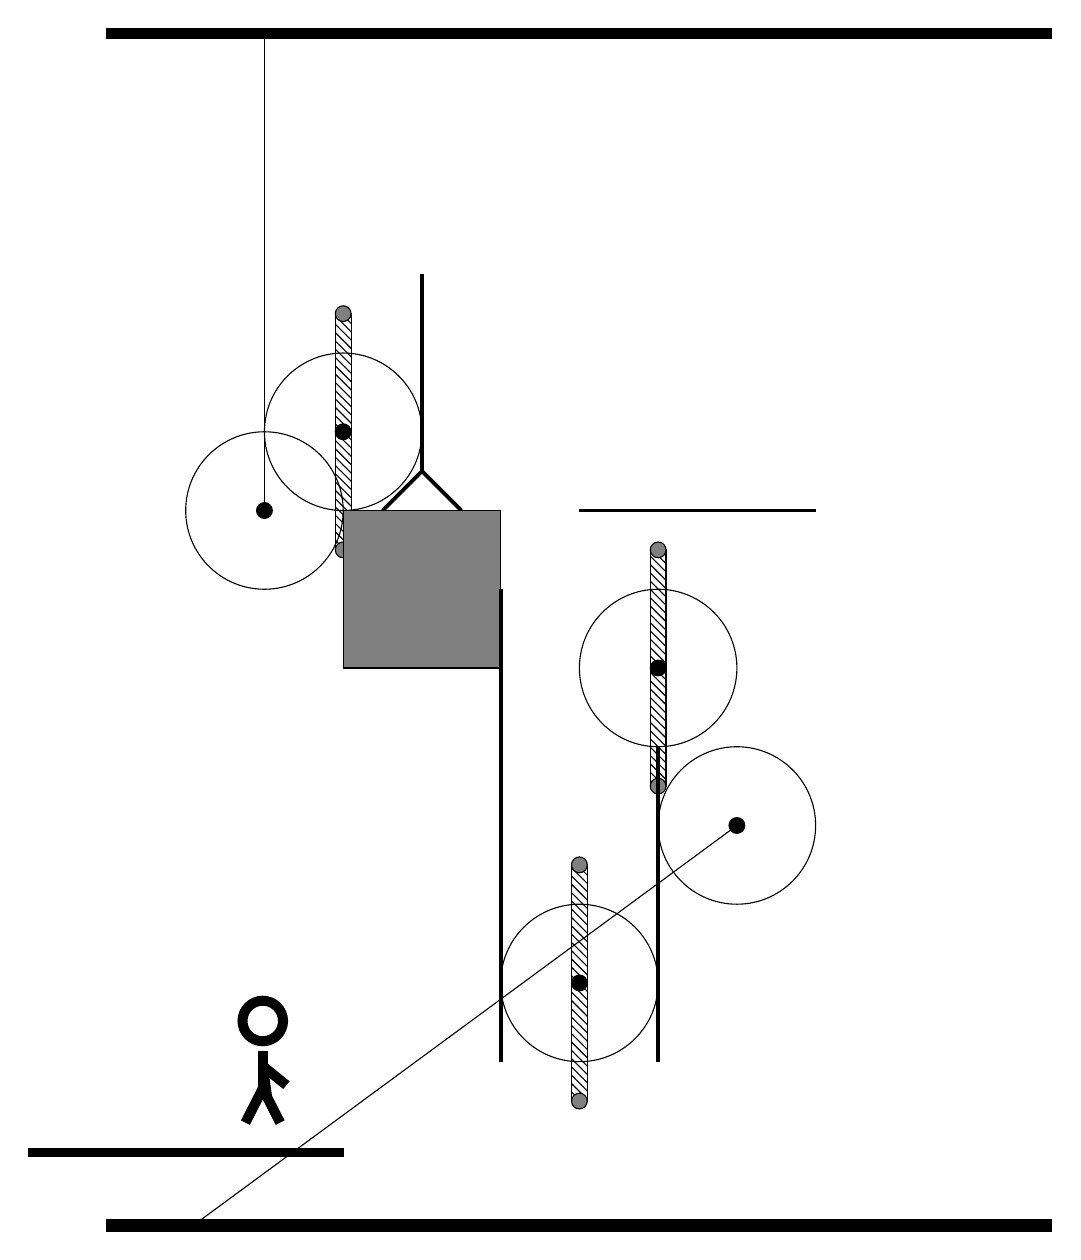
\begin{tikzpicture}
				\draw[fill=black] (-6, 12) rectangle (6, 12.125);
				
				\draw (-4,6) circle (1);
				\draw[fill=black] (-4,6) circle (0.1);
				\draw (-4,12.0) -- (-4,6);
				
				\draw (-3,7) circle (1);
				\draw[fill=black] (-3,7) circle (0.1);
				\draw[pattern=north west lines, pattern color=black] (-3.1,8.5) rectangle (-2.9,5.5);
				\draw[fill=black!50] (-3,8.5) circle (0.1);
				\draw[fill=black!50] (-3,5.5) circle (0.1);
				
				\draw (1,4) circle (1);
				\draw[fill=black] (1,4) circle (0.1);
				\draw[pattern=north west lines, pattern color=black] (0.9,5.5) rectangle (1.1,2.5);
				\draw[fill=black!50] (1,5.5) circle (0.1);
				\draw[fill=black!50] (1,2.5) circle (0.1);
				
				\draw (2,2) circle (1);
				\draw[fill=black] (2,2) circle (0.1);
				\draw (-5,-3.15) -- (2,2);
				
				\draw (0,0) circle (1);
				\draw[fill=black] (0,0) circle (0.1);
				\draw[pattern=north west lines, pattern color=black] (-0.1,1.5) rectangle (0.1,-1.5);
				\draw[fill=black!50] (0,1.5) circle (0.1);
				\draw[fill=black!50] (0,-1.5) circle (0.1);
				
				\draw[line width=0.5mm](-2,6.5) -- (-2,9.0);
				\draw[line width=0.5mm](-2.5,6) --  (-2,6.5) -- (-1.5,6);
				\draw[fill=black!50] (-3, 6) rectangle (-1, 4);
				
				\draw[line width = 0.5mm] (0,6) -- (3,6);
				\centerarc[line width = 0.5mm](0,5)(90:180:1);
				\draw[line width = 0.5mm] (-1,5) -- (-1,-1);
				\centerarc[line width = 0.5mm](0,-1)(180:360:1);
				\draw[line width = 0.5mm] (1,-1) -- (1,3);
				\centerarc[line width = 0.5mm](2,3)(0:180:1);
				
				\node at (-4, -1) {\scriptsize \Strichmaxerl[10][98][-39]};
				\draw[fill=black] (-7, -2.1) rectangle (-3, -2.2);
				
				\draw[fill=black] (-6, -3) rectangle (6, -3.15);
			\end{tikzpicture}
		\end{subfigure}
		\hfill
		\begin{subfigure}[b]{0.48\textwidth}
			\caption{Figure 2}
			\centering
			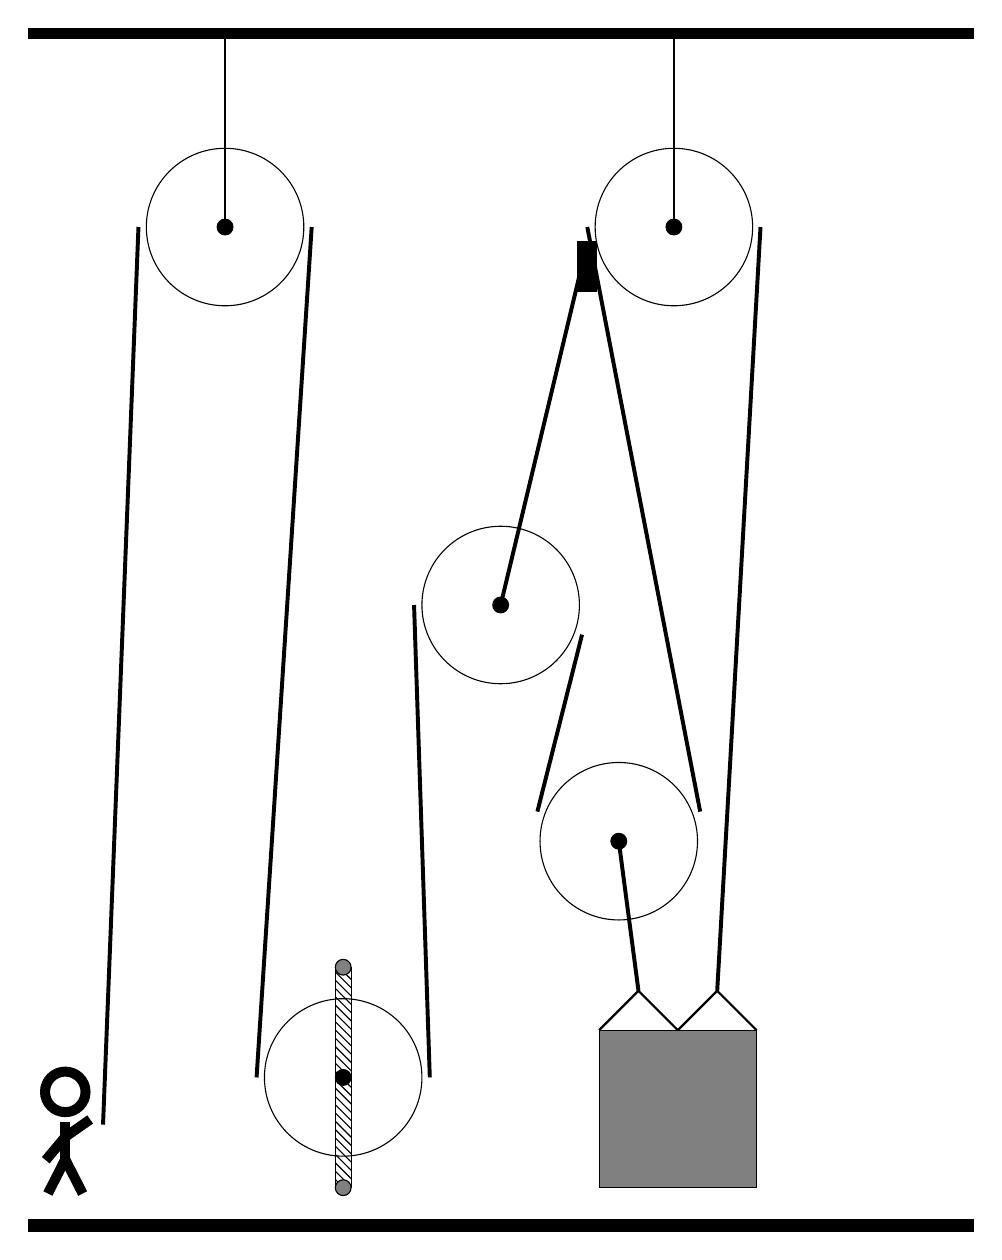
\begin{tikzpicture}
				\draw[fill=black] (-6, 12) rectangle (6, 12.125);
				
				\draw (0, 4.8) circle (1);
				\draw[fill=black] (0, 4.8) circle (0.1);
				
				\draw (1.5, 1.8) circle (1);
				\draw[fill=black] (1.5, 1.8) circle (0.1);
				
				\draw (2.2, 9.6) circle (1);
				\draw[fill=black] (2.2, 9.6) circle (0.1);
				\draw[thick] (2.2, 9.6) -- (2.2, 12);
				
				\draw (-3.5, 9.6) circle (1);
				\draw[fill=black] (-3.5, 9.6) circle (0.1);
				\draw[thick] (-3.5, 9.6) -- (-3.5, 12);
				
				\draw (-2, -1.2) circle (1);
				\draw[fill=black] (-2, -1.2) circle (0.1);
				\draw[pattern=north west lines, pattern color=black] (-2.1, 0.2) rectangle (-1.9, -2.6);
				\draw[fill=black!50] (-2, 0.2) circle (0.1);
				\draw[fill=black!50] (-2, -2.6) circle (0.1);
				
				\draw[thick]  (1.25, -0.6) -- (1.75, -0.1) -- (2.25, -0.6) -- (2.75, -0.1) -- (3.25, -0.6);
				\draw[fill=black!50] (1.25, -0.6) rectangle (3.25, -2.6);
				\draw[line width=0.5mm] (-5.05, -1.8) -- (-4.6, 9.6);
				\centerarc[line width=0.5mm](-3.5, 9.6)(0:180:1.1);
				\draw[line width=0.5mm] (-2.4, 9.6) -- (-3.1, -1.2);
				\centerarc[line width=0.5mm](-2, -1.2)(180:360:1.1);
				\draw[line width=0.5mm] (-0.9, -1.2) -- (-1.1, 4.8);
				\draw[line width=0.5mm] (0, 4.8) -- (1.1, 9.4);
				\draw[line width=0.5mm, fill=black](1.0, 8.8) rectangle (1.2, 9.4);
				\centerarc[line width=0.5mm](0, 4.8)(-20:180:1.1);
				\draw[line width=0.5mm] (1.0337, 4.4238) -- (0.4663, 2.1762);
				
				\centerarc[line width=0.5mm](1.5, 1.8)(160:380:1.1);
				\draw[line width=0.5mm] (2.5337, 2.1762) -- (1.1, 9.6);
				\draw[line width=0.5mm](1.5, 1.8) -- (1.75, -0.1);
				\centerarc[line width=0.5mm](2.2, 9.6)(0:180:1.1);
				\draw[line width=0.5mm] (3.3, 9.6) -- (2.75, -0.1);
				
				\node at (-5.5, -1.9) {\scriptsize \Strichmaxerl[10][50][35]};
				
				\draw[fill=black] (-6, -3) rectangle (6, -3.15);
			\end{tikzpicture}
		\end{subfigure}
	\end{figure}
		\vspace*{\fill}
\end{document}